\documentclass{article}

\usepackage{graphicx}
\usepackage{tikz}
\usepackage{tikzsymbols}
\usetikzlibrary{calc,patterns,shapes.geometric}
\pagestyle{empty}
\usepackage[margin=0pt]{geometry}
\geometry{papersize={14in,12in}}

\def\centerarc[#1](#2)(#3:#4:#5){\draw[#1] ($(#2)+({#5*cos(#3)},{#5*sin(#3)})$) arc (#3:#4:#5);}

\begin{document}
	\begin{figure}
		\centering
		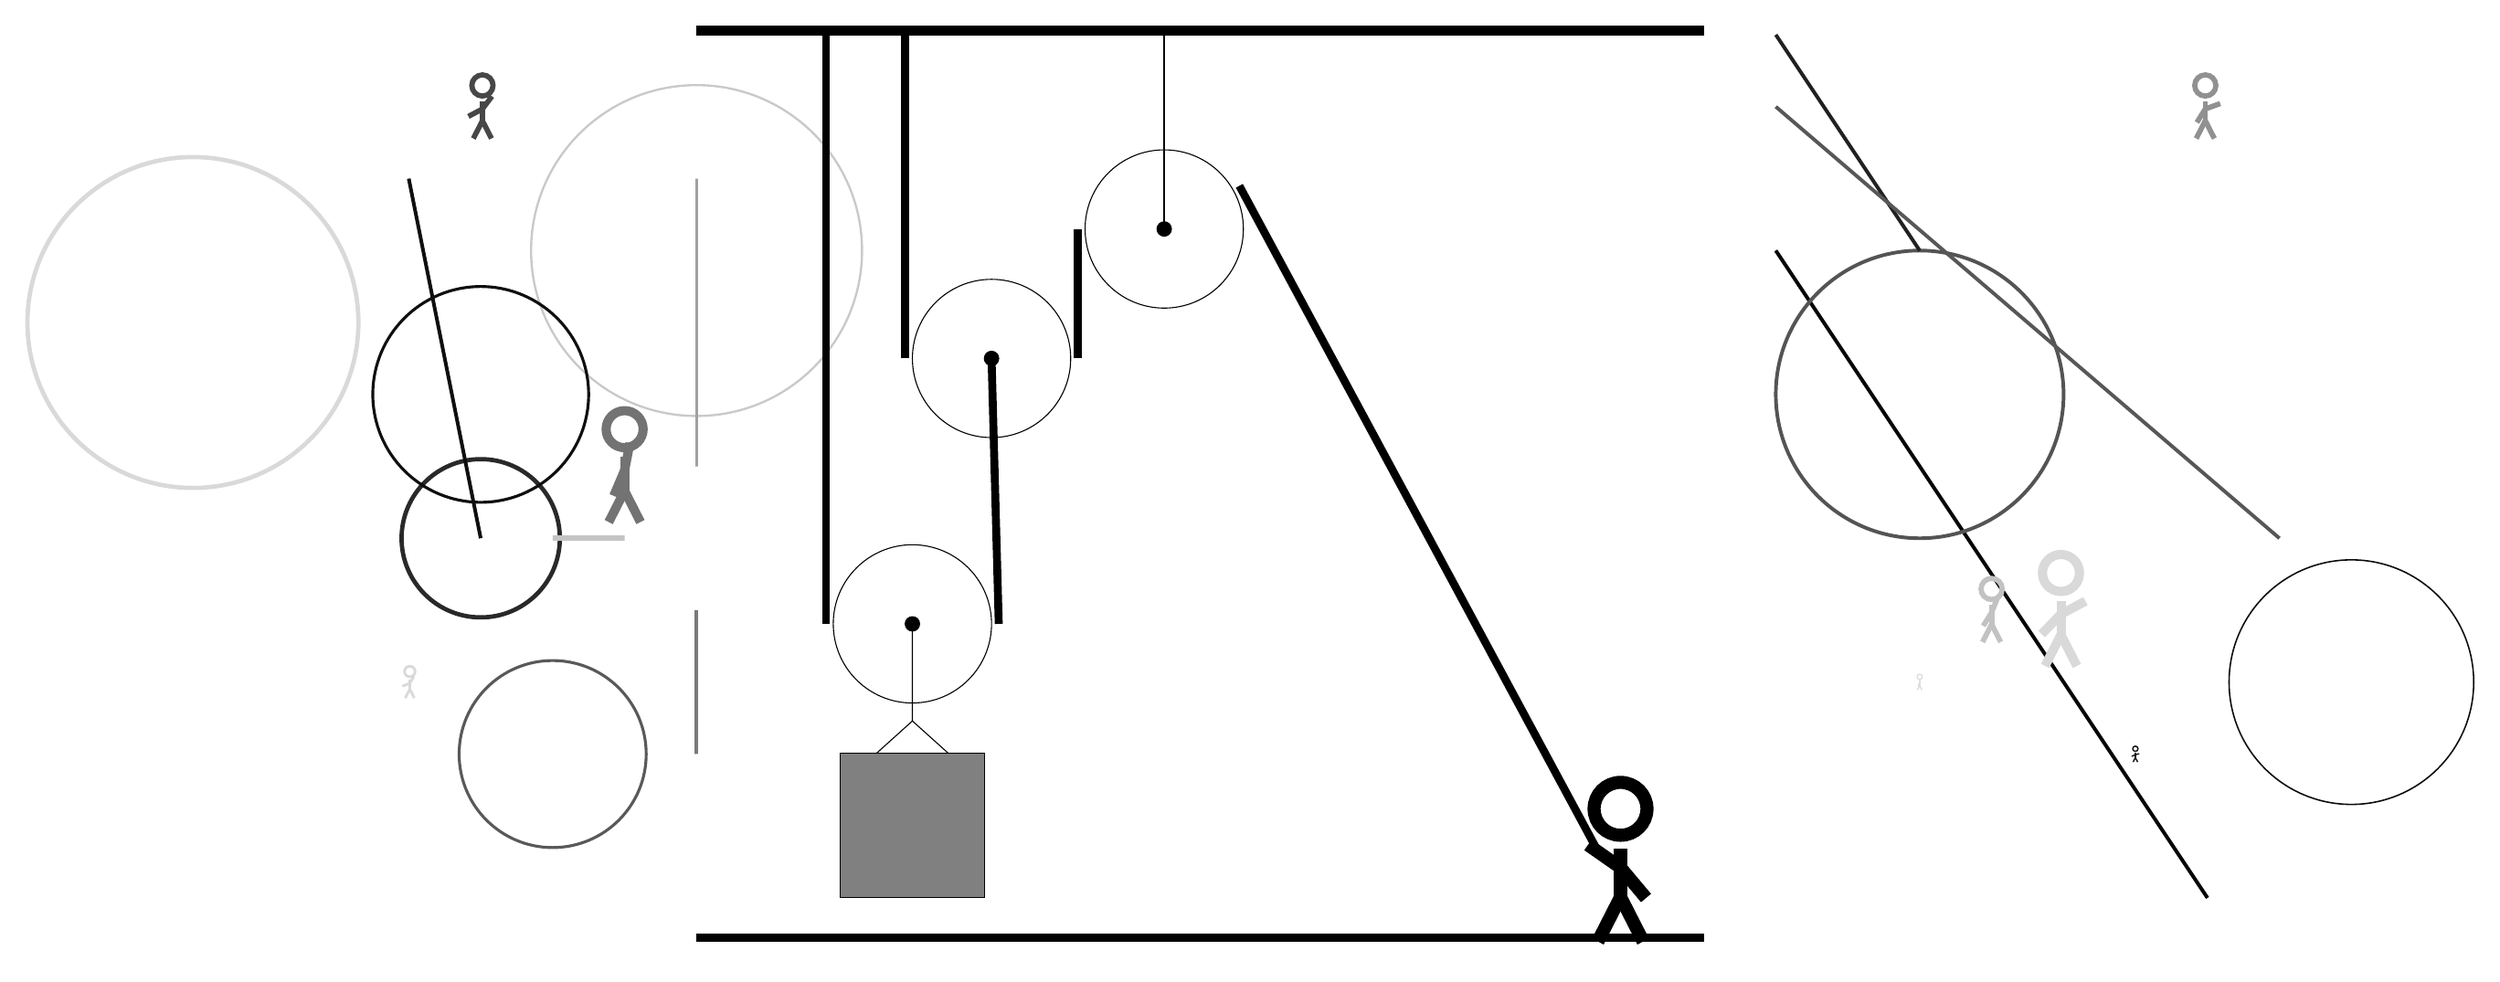
\begin{tikzpicture}
			%%%%% START %%%%%
			
			\draw[fill=black] (-2, 9) rectangle (12, 9.125);
			
			\draw (1, 0.81) circle (1.1);
			\draw[fill=black] (1, 0.81) circle (0.1);
			
			\draw (2.1, 4.5) circle (1.1);
			\draw[fill=black] (2.1, 4.5) circle (0.1);
			
			\draw (4.5, 6.3) circle (1.1);
			\draw[fill=black] (4.5, 6.3) circle (0.1);
			\draw[thick] (4.5, 6.3) -- (4.5, 9);
			
			\draw [line width=0.6mm, color=black!84](-5, 2) circle (1.1);
			
			\draw[line width=0.5mm, color=black!52] (-2, 1) rectangle (-2, -1);
			\draw[line width=0.7mm, color=black!23] (-4, 2) rectangle (-3, 2);
			\draw[line width=0.5mm, color=black!98](13, 6) -- (19, -3);
			\node[line width=0.7mm, color=black!24] at (16, 1) {\Strichmaxerl[4][58][68]};
			\node[line width=0.3mm, color=black!55] at (-3, 3) {\Strichmaxerl[7][67][79]};
			\node[line width=0.5mm, color=black!93] at (18, -1) {\Strichmaxerl[1][26][13]};
			\node[line width=0.2mm, color=black!72] at (-5, 8) {\Strichmaxerl[4][28][53]};
			\draw [line width=0.4mm, color=black!65](-4, -1) circle (1.3);
			\draw [line width=0.6mm, color=black!15](-9, 5) circle (2.3);
			\draw [line width=0.3mm, color=black!21](-2, 6) circle (2.3);
			
			\draw [line width=0.2mm, color=black!96](21, 0) circle (1.7);
			\node[line width=0.4mm, color=black!43] at (19, 8) {\Strichmaxerl[4][58][20]};
			\draw [line width=0.5mm, color=black!67](15, 4) circle (2.0);
			\node[line width=0.4mm, color=black!15] at (-6, 0) {\Strichmaxerl[2][22][59]};
			\draw [line width=0.4mm, color=black!94](-5, 4) circle (1.5);
			
			\draw[line width=0.4mm, color=black!37] (-2, 7) rectangle (-2, 3);
			
			\node[line width=0.4mm, color=black!15] at (17, 1) {\Strichmaxerl[7][46][28]};
			\draw[line width=0.5mm, color=black!87](13, 9) -- (15, 6);
			\draw[line width=0.5mm, color=black!94](-6, 7) -- (-5, 2);
			\node[line width=0.4mm, color=black!13] at (15, 0) {\Strichmaxerl[1][65][83]};
			
			\draw[line width=0.5mm, color=black!66](13, 8) -- (20, 2);
			
			\draw (1, 0.81) -- (1, -0.54) -- (0.5, -0.99) -- (1.5, -0.99) -- (1, -0.54);
			\draw[fill=black!50] (0, -0.99) rectangle (2, -2.99);
			
			\draw[line width=1.1mm] (-0.2, 9) -- (-0.2, 0.81);
			\centerarc[line width=1.1mm](1, 0.81)(180:360:1.2000000000000002);
			\draw[line width=1.1mm](2.2, 0.81) -- (2.1, 4.5);
			\draw[line width=1.1mm] (0.9, 9) -- (0.9, 4.5);
			\centerarc[line width=1.1mm](2.1, 4.5)(180:360:1.2000000000000002);
			\draw[line width=1.1mm](3.3, 4.5) -- (3.3, 6.3);
			\centerarc[line width=1.1mm](4.5, 6.3)(30:180:1.2000000000000002);
			\draw[line width=1.1mm] (5.544, 6.9) -- (10.5, -2.3);
			
			\node at (10.8, -2.5) {\Strichmaxerl[10][-35][-50]};
			
			\draw[fill=black] (-2, -3.5) rectangle (12, -3.6);
			
			%%%%% END %%%%%
		\end{tikzpicture}
	\end{figure}	
\end{document}